\documentclass[a4paper,10pt]{report}

\usepackage[utf8]{inputenc}
\usepackage{xspace}
\usepackage{graphicx,graphics} 
\usepackage{color}
\usepackage{amsmath}
\usepackage{amsfonts}
\usepackage{amssymb}
\usepackage{amsthm}
\usepackage{algorithm}
\usepackage{algorithmic}
\usepackage{longtable}
\usepackage{complexity}

\graphicspath{{figures/}}
\newcommand\rmatching{$\cal R$-matching\xspace}
\newcommand\mdelay{$\cal M$-delay\xspace}
\newcommand\matchedgraph{{\bf matched graph}}
\begin{document}
\begin{chapter}{Context, company and subject}
\begin{section}{Company}
 Description de Nokia Bell Labs, Activité dans les équipements télécoms. (Voir avec Olivier)
\end{section}
\begin{section}{Context}
 Utiliser le sujet de these : C-RAN pour 5g. Centralisation des BBU à travers les réseaux fronthaul.
 Fortes contraintes en débit et en latence. Expliquer le sujet : trouver des algorithme qui permettent de faire 
 transiter les messages sans contentions dans les switchs.
\end{section}

\end{chapter}

\begin{chapter}{Problem, model}
 \begin{section}{Model}
 \begin{subsection}{Definitions}
  A Fronthaul network can be considered as a directed graph $G=(V,A)$ with two non intersecting subsets of vertices: 
  a subset $L$ of nodes which are called  \emph{leaves} and a subset $S$ of nodes which are called \emph{sources}.  
The indegree of nodes in $S$, and the outdegree of nodes in $L$ are equal to 0. 
We denote by ${\cal L}$ the cardinal of $L$ and by ${\cal S}$ the cardinal of $S$. The digraph $G$ models the network,
$S$ is the set of BBU and $L$ is the set of RRH. The others nodes of the graph are the switches.
Each arc  $(u,v)$ in $A$ has an integer weight $Dl(u,v) \geq 1$ representing the time taken by the signal to go from $u$ to $v$
by using this arc. This is the physical delay of a link.

We consider $G^r=(V,A^r)$ wherein the set of vertices is the same as in $G$, and $A^r$ represents the edges of $A$ directed in the other way. 
\newline
\begin{tabular}{cc}
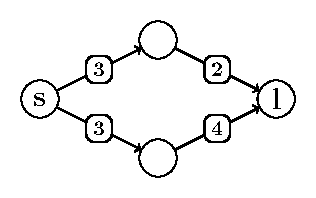
\includegraphics[scale=0.8]{Fig2.pdf} & 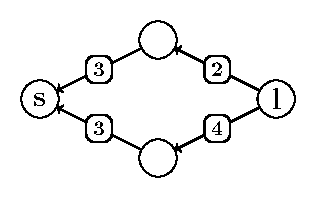
\includegraphics[scale=0.8]{Fig3.pdf}\\
 $G=(V,A)$ & $G^r=(V,A^r)$\\
\end{tabular}\newline

A {\bf route} $r$ is a sequence of arcs $a_0, \ldots , a_{n-1}$, with $a_i=(u_i,u_{i+1}) \in A$ such that $u_0 \in S$ and $u_n \in L$.
The {\bf latency} of a vertex $u_i$ in $r$, with $i \geq 1$, is defined by $$\lambda(u_i,r)= \sum\limits_{0 \leq k <i} Dl(a_k)$$ We also define $\lambda(u_0,r)=0$.
The latency of the route $r$ is defined by $\lambda (r)= \lambda (u_n,r)$. In graph theory, a route is a simple path in the graph, and its latency is its weight. 


A {\bf routing function} ${\cal R}$ is an application associating a route ${\cal R}(s,l)$ to each couple $(s,l) \in S \times L$ in $G$.
Moreover ${\cal R}$ satisfies the \emph{coherent routing} property: the intersection of two routes must be a path.

For simplicity, we assume that we have as many source nodes as we have leaves (${\cal S} = {\cal L})$.
A {\bf ${\cal R}$-matching} is a bijection $\rho :S\rightarrow L$ which associates to each $s_i \in \{s_0,...,s_{{\cal S}-1}\}$ 
a $l_i \in \{l_0,...,l_{{\cal L}-1}\}$.
A \rmatching defines a set $\{r_0, \ldots ,r_{{\cal L}-1}\}$ of ${\cal L}$ routes in R such that $\forall i\,, r_i = R(s_i,l_i)$.

The quintuplet $N=(G,S,L,R,\rho)$ defines a \matchedgraph. We call $N^r$ the quintuplet $(G^r,S,L,R,\rho^r)$, 
where $\rho^r$ is the \rmatching obtained using the same routes, with inverted arcs.

\end{subsection}
\begin{subsection}{Slotted time Model}
Consider the time split in {\bf time slots}. A time, expressed in slots, represents either the emission time of a message by a node ({\bf message length}),
or the time taken by a message to cross a link (this is the delay of an arc).
Let $P>0$ be an integer called {\em period}. 
A $P$-periodic affectation of N, a matched graph consists in a set  ${\cal M}=(m_0, \ldots ,m_{{\cal L}-1})$
of ${\cal L}$ integers that we call \emph{offset}. 
Each time window is divided in $P$ slots and the number $m_i$ represents the first slot number used by the route $r_i$ at its source.
We define the first time slots used by a route $r_i$ at any vertex $v$ of the route by $$t(v,r_i) = m_i+\lambda(u,r_i)) \mod P.$$
Each route is using an interval $[t(v,r_i);t(v,r_i)+T_i]$ in each vertex $v$, where $T_i$ is the message length of the message transiting on the route i.

A $P$-periodic affectation must have no {\em collision} between two routes in $\rho$, that is $\forall r_i, r_j \in \rho, i \ne j$,
two routes intersecting in u, and containing the same arc $(u,v)$, we have $$t(u,r_i)\ne t(u,r_j) .$$

\fbox{\parbox{12cm}{
Notice that the notion of $P$-periodic affectation \textbf{is not monotone} with regard to $P$. 
Indeed, we can build a {\bf ${\cal R}$-matching} of a graph, with ${\cal L}$ routes $r_1, \dots, r_l$ which all intersect two by two and
such that if $r_i$ and $r_j$ have $v$ as first common vertex we have $\lambda(v,r_i) - \lambda(v,r_j)=1$.
Therefore there is a $2$-periodic affectation by setting all $m_i$ to $0$.

\begin{tabular}{cc}
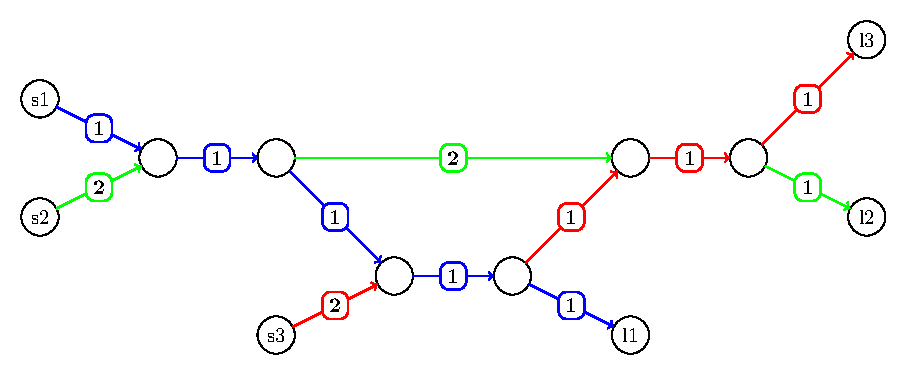
\includegraphics[scale=0.5]{Fig5.pdf} & 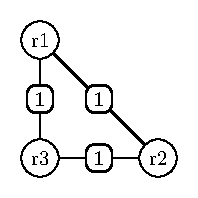
\includegraphics[scale=1]{Fig7.pdf}\\
 $\lambda(v,r_i) - \lambda(v,r_j)=1$ & Conflict graph\\
\end{tabular}\newline

On the other hand if we set all $\lambda(v,r_i) - \lambda(v,r_j)=P$, there is no $P$-peridodic affectation if $P<l$.

\begin{tabular}{cc}
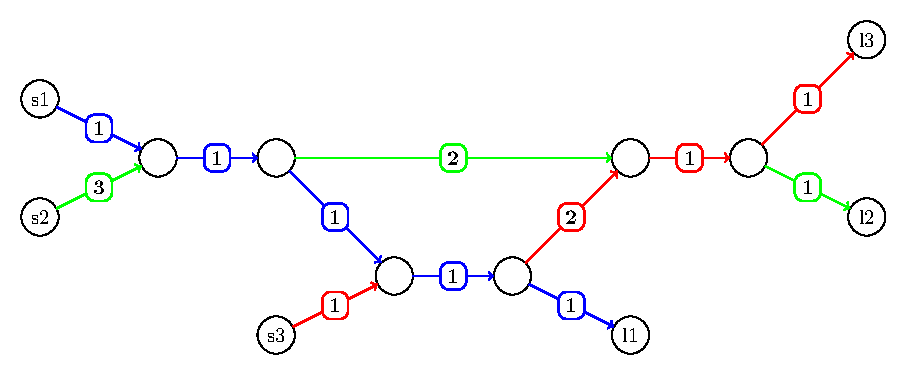
\includegraphics[scale=0.5]{Fig6.pdf} & 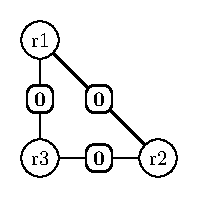
\includegraphics[scale=1]{Fig8.pdf}\\
 $\lambda(v,r_i) - \lambda(v,r_j)=2$ & Conflict graph\\
\end{tabular}\newline
\begin{center}
 Here for P=2, there is no P-Periodic affectation.
\end{center}

Therefore if we choose $P$ odd and $l=P+1$, there is no $P$-peridodic affectation but modulo $2$ all $\lambda(v,r_i) - \lambda(v,r_j)$
are equal to one thus we have a $2$-periodic affectation. 
}}
\end{subsection}
\begin{subsection}{Topology}

We consider 3 kinds of topologies corresponding to the different kinds of fronthaul networks: 
\begin{enumerate}
 \item Topology 1 : a basic network topology, composed of some base stations, represented by source nodes $S$, all connected to the same switch,
which will be a vertex, connected himself to another vertex, corresponding to a switch, connected to some leave nodes $L$ representing the Antennas.
\item Topology 2 : A network containing an optical ring, such that some sources nodes may join it anywhere, not intersecting themselves before the ring,
and some set of leave nodes are also leaving at any point of the ring.
\item Topology 3 : A ''random`` network, generated with some realistic properties (number of vertices, degree ...)
\end{enumerate}

This report focus on studying the first topology, which looks trivial but in fact, causes many issues.

\end{subsection}

\end{section}
\begin{section}{Problem}
   
The application we address here by studying the problems defined above is the following. Consider a fronthaul network in which source nodes in $S$ represent computing units in data centers,
each one able to do a remote process for base stations represented by leaves node in $L$. Consider a ${\cal R}$-matching $\rho$ of $S$ in $L$. Consider a leaf $l$, its dedicated source node $s$
and $R(l,s)$ the route from $l$ to $s$ in $R$. We consider a $P$-periodic affectation of N, and also another $P$-periodic affectation of N$^{r}$.
The periodic process is then the following one:
\begin{enumerate}
 \item During each period of duration $P$, $l$ sends a message to its dedicated source $s$, using their dedicated routes and considering the $P$-periodic affectation of N. 
 \item When each $s$ receives this message, it makes a computation to answer $l$. This computation time is fixed.
 \item After this computation time, $s$ sends a message to $l$ considering the $P$-periodic affectation of N$^{r}$.
\end{enumerate}
On source nodes, between the end of computation time and the emission time of the message (given by the $P$-periodic affectation), there is a $waiting\:time$. 
We define by $\omega : r \rightarrow \mathbb{N}$ the waiting time of a route $r$ in the ${\cal R}$-matching considered, i.e. the time during which the
message is ''sleeping``, waiting to be sent through the network.


Source and leave nodes periods have to be the same. Indeed, leave nodes have to receive a message at every period, so source nodes have to send a message at every same period.
So, we will find two P periodic affectations from the same P in both ways. 
If the messages have to be buffered, we want to do it in sources nodes.
We define by $\theta$ the computation time required at the source node before sending an answer to it's leave node.

Let us call $T (r)$ the process time on a route $r$: $$ T (r) = 2\lambda (r) + \omega (r) + \theta$$

Since $\theta$ is the same on every routes, we can simplify the model by removing this $\theta$.Whether we want to consider it, we only have to lengthen all 
links before source nodes from an integer corresponding to $\theta$. 


In our network application, as $P$ and the $R-matching$ are given, we do not need to minimize $P$ because generally $P$ is big enough to carry the dataload.
Therefore we want to optimize the time taken by the messages to do the two way trip in order to ensure a good level of quality of service.

A {\bf 2-way-trip affectation} of $N$ is a set of doublets $ ((x_0,m_0),...,(x_{{\cal L}-1},m_{{\cal L}-1}))$ in which ${\cal M} = (m_0,...,m_{{\cal L}-1})$ 
is a $P$-periodic affectation of N$^r$,and $x_i$ is calculated as following :
$$ x_i = ( m_i + \lambda(r_i) + \theta + \omega_i ) mod P $$
where ${\Omega} = (\omega_0,...,\omega_{{\cal L}-1}) $ is the $P$-periodic affectation of N. This means that $\forall i,j,x_i \notin [x_j,...,x_j+T]$, to avoid collisions
.$T$ is the size of the message.

Note that i design the route and that the second $P$-periodic affectation ${\Omega}$ correspond to the waiting times of routes : $\omega_i = \omega(r_i)$.

Our real network problem is the following:\\

\noindent {\bf Problem Periodic Assignment for Low Latency(PALL)} 

\noindent {\bf Input:} matched graphs $N$, integer $P$, $ T_{max}$.

\noindent {\bf Question:} does there exist a 2-way-trip affectation of $N$, such that $\forall r \in \rho$, $T(r) \le T_{max}$.

\noindent {\bf Optimization goal 1:} minimizing max(T(r)).\\

Minimizing the more expensive in time of all routes allows to ensure that any route will exceed the deadline of 3ms.

\noindent {\bf Optimization goal 2:} minimizing $\sum_{r \in \rho}  T(r)$ (equivalent to minimizing $\sum_{r \in \rho}  \omega(r)$.\\

By minimizing the sum of all the routes, we allow a better global Quality of Service trough the network.\\
\begin{subsection}{Different cases}
\begin{center}
 
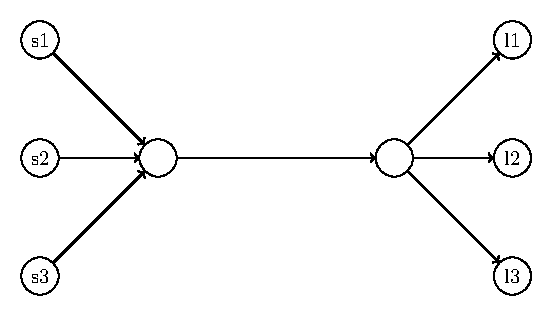
\includegraphics[scale=1]{Fig4.pdf}\\
Example of topology 1.
\end{center}



In the considered topology, there is 3 cases :
\begin{itemize}
 \item 1: When the weight of the links from source nodes are all equal. This is the closest case to the reality, but also the easier to solve.
 \item 2: When the weight of the leave nodes links are all equal .
 \item 3: When all the links have different weights.
\end{itemize}
The middle link can be represented without weight, because it is common to all the routes, so it can be simplified in calculations. 
Likewise, we do not consider $\theta$, the calculation time.

\end{subsection}
\end{section}
\begin{section}{Related Work}
\begin{subsection}{Path Colouring and Call Scheduling}
I have studied an article of Thomas Erlebach and Klaus Jansen about the Path coloring and Call Scheduling \cite{erlebach2001complexity}.
Those two Methods are similar to our problem.

\paragraph{Path Coloring}
The path coloring works on all optical networks. It tries to establish a connection between two nodes, by reserving a wavelength on all links of the
path between the two nodes. The number of wavelengths is limited, so it is necessary to find a way to use the minimum number of wavelength for a set 
of connections.

The model used is a graph $G=(V,E)$ in which the vertex represent the switches and the links are modeled by the edges. The goal is to give to each
couple of vertex (u,v), a path and a color representing the connection, such that any other couple using a common edge in it's path has the same
color than (u,v). The problem is to minimise the number of color used.

Applied to our problem, path coloring return to give a different color to each couple BBU/RRH, because they all share the same common link.


\paragraph{Call Scheduling}
The call scheduling is applied to bandwidth reservation networks. In these networks, the links had different bandwidth and every message 
requires a certain bandwidth reservation. The problem is to set the paths and the starting times of the connection requests.
The goal is to minimise the latest completion time i.e. the moment in which all the messages are transmitted.

To solve this problem, the authors are using a graph $G=(V,E)$, in which the edges gets a capacity representing the bandwidth.
A call is represented by a couple (u,v) of vertex, a bandwidth requirement and a duration. The goal is to give a starting time to each call
such that any call has enough bandwidth on it's links when it is active.

Our problem is a simplified cases of the call scheduling because all the bandwidth requirement, call duration and edge capacities are the same.
Solving call scheduling doesn't solve our two way trip problem, it just helps us to find a solution for the first P-peridodic affectation.

Further, this article does not give an algorithm to solve path coloring or call scheduling.

\end{subsection}

\begin{subsection}{Barbara Simons}
 \cite{simons1978fast}
\end{subsection}

Résumé des articles Simons et Path coloring/Call Scheduling.
Parler du passage du Garey and Johnson sur la complexité.
 \end{section}


\end{chapter}

\begin{chapter}{Algorithms and studies }


\begin{section}{First approach : without waiting times}
 Présentation des différents algos (celui avec des certitudes théoriques, le bruteforce et l'algo sur lequel on n'a pas d'analyse) pour trouver 
 une solution sans waiting times. Ne pas hesiter a mettre les exemples de l'article qui prouvent que le waiting time est nécéssaire avec notre contrainte de temps.
 \end{section}

\begin{section}{Main Algorithm}
Description du fonctionnement de l'algo longest shortest et Simons sur notre modèle. Expliquer pourquoi sur notre problème ils sont equivalents.
 Résultats théoriques sur les différents cas de la topologie 1. Ici expliquer que les cas 1 et 2 sont triviaux, et qu'on ne traite désormais que le 
 cas global.
\end{section}

\end{chapter}

\begin{chapter}{Simulations}


\begin{section}{Pour chaque courbe}
\begin{itemize}
 \item Données en entrées, Lois utilisées.
 \item Métrique, donnée mesurée, algos comparés, nombre de simuls.
 \item Resultats, commentaires infos importante que l'on conclus.
\end{itemize}
\end{section}

\begin{section}{No waiting time involve bigger periods}
Ici montrer le graph de la taille des fenêtres pour les algos sans waiting time.
 En conclure que le bruteforce est le mieux
\end{section}

\begin{section}{Limits of ``Nom que je donne au bruteforce''}

 Résultats de simulations qui montrent à partir de quelle charge du réseau le bruteforce nous indique qu'il n'y 
 a plus de solutions sans waiting time.
Conclusion : utilité d'algos dans lesquels on autorise les waiting times
\end{section}

\begin{section}{Longest Shortest}
Montrer que simons = longest shortest sur toutes nos instances.
Graphique des $T_{max}$ pour l'algo longest shortest et random.
Montrer que les résultats sont très bon pour longest shortest et très mauvais pour random dès que le charge dépasse un certain seuil.
Montrer aussi les distributions cumulées qui montrent une nouvelle fois que le longest shortest est utile.
\end{section}

\begin{section}{Synthesis}
Reprendre tous les résultats
\end{section}

\end{chapter}



\begin{chapter}{Conclusion}
\begin{itemize}
 \item Comprendre le problème (parler de l'article qui à été faite avant par DAVID sur le sujet)
 \item Lecture des articles, définition du modèle
 \item Simulations
 \item résultats, utilisables sur les autres topologies ?...
\end{itemize}



\end{chapter}


\bibliographystyle{plain}
\bibliography{Sources}

\end{document}


































































































































































































































































































































































































































































































































































































































































































































































































































































































































































































































































































































































































































































































































































































































































































































































































































































































































































































































































































































































































































































































































































































































































































































































































































































































































































































































































































































































































































































































































































































































































































































































































































































































































































































































































































































































































































































































































































































































































































































































































































































































































































































































































































































































































































































































































































































































































































































































































































































































































































































































































































































































































































































































































































































































































































































































































































































































































































































































































































































































































































































































































































































































































































































































































































































































































































































































































































































































































































































































































































































































































































































































































































































































































































































